\documentclass{article}

\usepackage[ngerman]{babel}
\usepackage{siunitx}
\usepackage{graphicx}

\begin{document}
\section*{Aromaten}
Die Moleküle aromatischer Kohlenwasserstoffe sind ebene (planare)
Ringe mit konjugierten Doppelbindungen. Um die Strukturformeln darstellen zu können 
verwendet man Mesomere.
\subsection*{Benzol}
\subsubsection*{Struktur}
Benzol besitzt die Strukturformel ($C_6H_6$). Kekule vermutete die Strukturformel des
Benzols als Cyclohexa-1,3,5-trien. Jedoch zeigen Röntgenstrukturanalysen, dass alle 
Bindungslängen gleich lang sind. In wahrheit überlappen sich die p-Orbitale des freien
Elektrons der C-Atome und bilden ein $\pi$ Elektronensystem. Die Elektronen sind 
\emph{delokalisiert}. Dies lässt sich auch durch die frei werdende Bindungsenergie bei
der Reaktion von Benzol zu Cyclohexan belegen. Bei der Reaktion von Cyclohexen zu 
Cyclohexan werden 120 \unit{kJ} frei. Somit sollten bei der Reaktion vom hypothetischen
Cyclohexa-1,3,5-trien 360 \unit{kJ} frei werden. Jedoch werden nur 209 \unit{kj} frei.
Dies legt nahe, dass sich das Benzol in einem energetisch günstigern Zustand befindet.
Benzol reagiert auch mit Brom nicht wie normalerweise mit einer Additionsreaktion,
sondern mit einer Substitutionsreaktion. Dies ist der Fall, da so der energetisch günstige Zustand des 
Benzols nicht zerstört wird.

\subsubsection*{Eigenschaften}
\begin{itemize}
    \item aromatischer Geruch
    \item brennbar (rußt stark)
    \item hydrophob
    \item stark lichtbrechend
    \item Dichte $ > 1 \frac{\unit{g}}{\unit{ml}} $
    \item giftig / krebserregend
\end{itemize}
\section*{Toxizität}
\subsection*{$LD_{50}$}
Der $LD_{50}$-Wert beschreibt die letale Dosis eines Stoffes, bei der 50\% der Versuchstiere
sterben [\unit{mg}/\unit{kg} Körpergewicht]
\subsection*{AGW (Arbeitsplatzgrenzwert)}
maximale Konzentration eines Gefahrstoffs in der Luft am Arbeitsplatz [\unit{mg}/\unit{m^3}] 
\section*{Kunststoffverwertung}
\subsection*{werkstoffliche Verwertung}
$\approx 46\%$\newline
Kunststoffe werden gereinigt, zerkleinert und eingeschmolzen. Beispiel: PET-Flaschen\newline
sortenreine Kunststoffe $\rightarrow$ Kunststoffgranulat $\rightarrow$ gemischte Downcycling-Kunststoffe
$\rightarrow$ Fertigprodukt
\subsection*{rohstoffliche Verwertung}
$\approx 1\%$\newline
Polymere werden durhc chemische/biologische Verfahren in Monomere zerlegt. Beispiel: Enzym-Reaktion\newline
Hydrolyse/Soluolyse/enzymatische Prozesse $\rightarrow$ Makromoleküle werden zerlegt $\rightarrow$ Monomere
\subsection*{energetische Verwertung}
$\approx 53\%$\newline
Verbrennung und Energiegewinnung in Verbrennungs/Betonwerken\newline
Makromoleküle werden zerlegt$\rightarrow$Energie/Strom
\section*{Verarbeitungsverfahren von Kunststoffen}
\subsection*{Extrusion}
\begin{itemize}
    \item Granulat wird durch Heizung und Schnekenreibung geschmolzen
    \item Schnekcke zieht scih zurück, um Druch auszugleichen
    \item SChnecke wird hydraulisch nach vorne gedrückt und presst das geschmolzene Granulat
    durch das gkühlte Werkzeug
\end{itemize}
Leisten, Kabel
\subsection*{Spritzgießen}
\begin{itemize}
\item Kunststoffstrang wird durch Extruder in Form gepresst 
\end{itemize}
Autoteile
\subsection*{Folienblasen}
\begin{itemize}
    \item Kunststoffstrang wird durch Luftzug gestreckt und die nun dünnen Seile werden zu
    einer Folie zusammengelegt
\end{itemize}
Plane
\subsection*{Prssen}
\begin{itemize}
    \item Rohstoffe kommen verbrauchsfertig hinein und werden in Form gepresst
\end{itemize}
Tupperware, Geschirr
\subsection*{Blasfromverfahren, Schlauchform}
\begin{itemize}
    \item weicher Kunststoffschlauch wird in Blasform gelegt 
    \item Schlauch wird aufgeblasen
    \item überschüssiges Material wird abgeschnitten
\end{itemize}
Flaschen
\subsection*{Kalandrieren}
\begin{itemize}
    \item Masse wird über viele Walzen gezogen und gereckt (durch ziehen dünner) 
\end{itemize}
Blisterfolie
\subsection*{3D-Druck}
\begin{itemize}
    \item Objekt wird schichtweise durch geschmolzenes Filament aufgebaut
\end{itemize}
\section*{Wichtige Moleküle}
\subsection*{Benzoesäure}
\includegraphics[width=0.25\textwidth]{Benzoesäure.png}
\subsection*{Terephtalsäure}
\includegraphics[width=0.25\textwidth]{Terephtalsäure.png}
\subsection*{Phenylalanin}

\includegraphics[width=0.25\textwidth]{Phenylalanin.png}
\subsection*{Styrol}
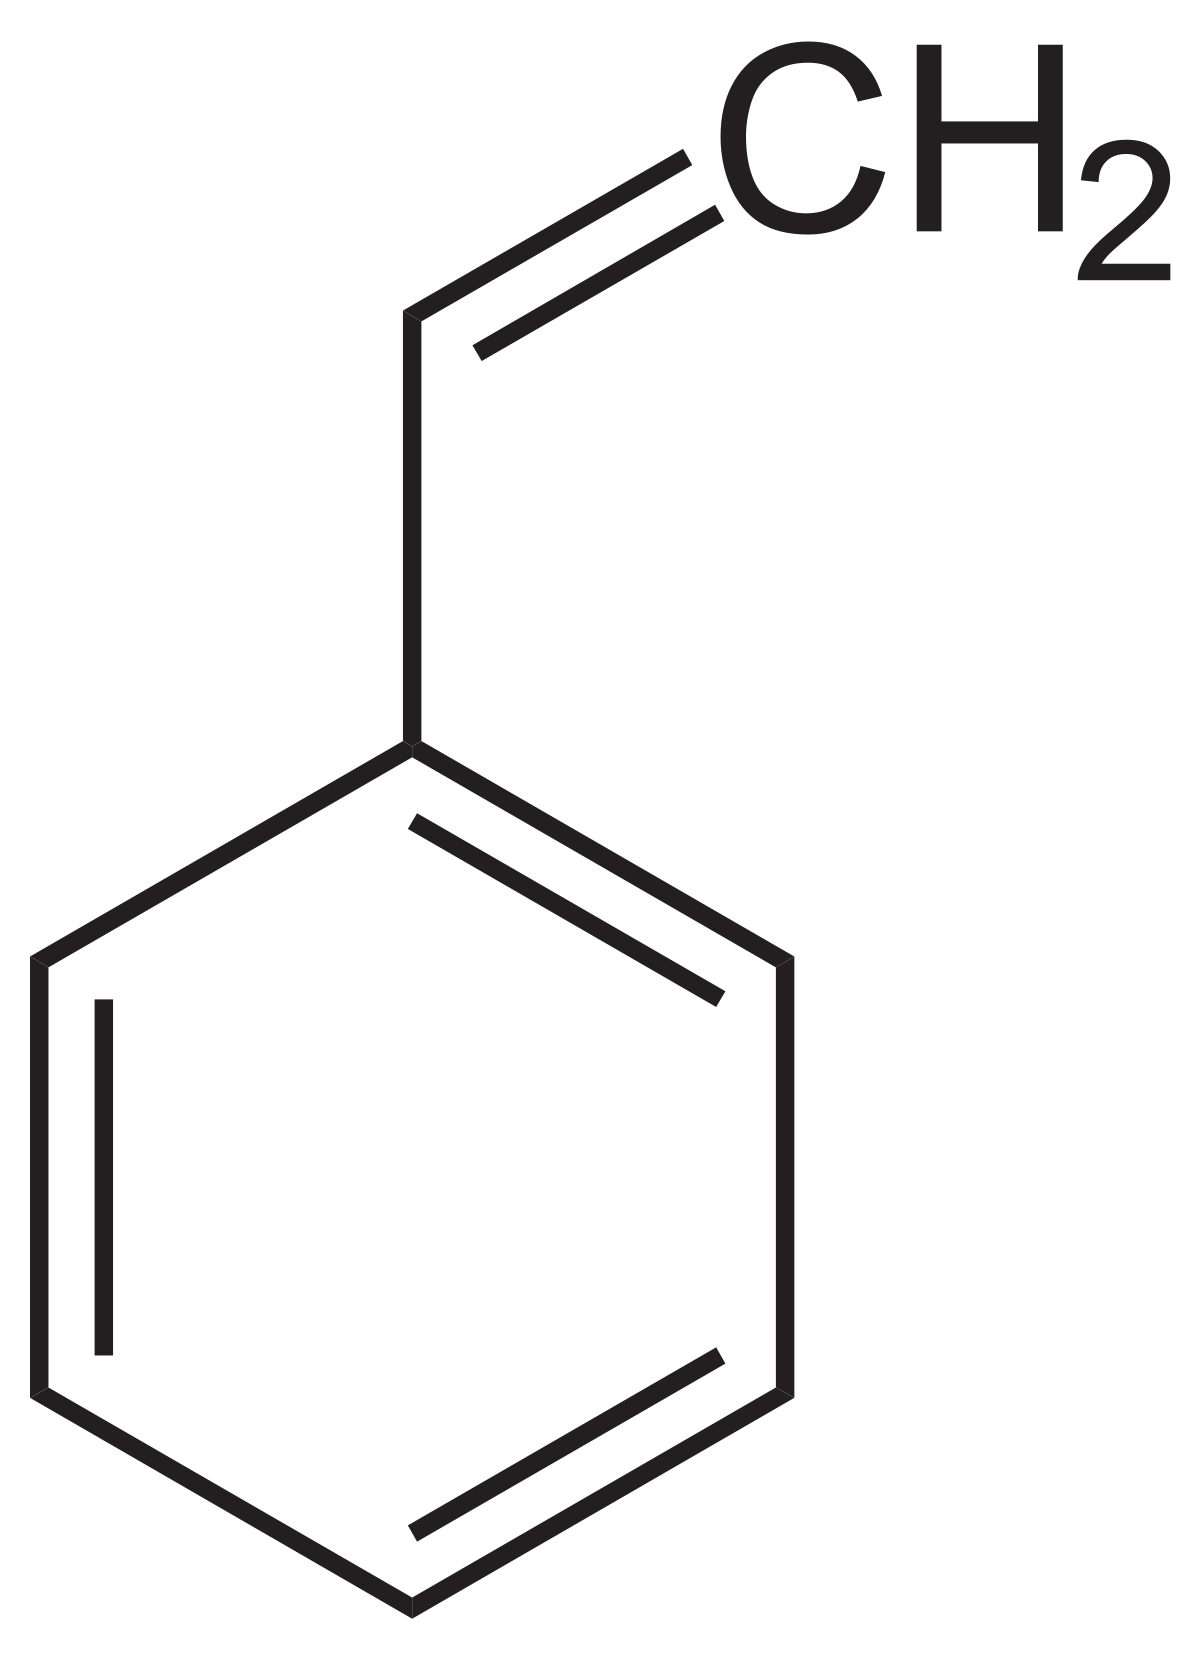
\includegraphics[width=0.25\textwidth]{Styrol.png}
\end{document}